\documentclass[a4paper,twoside]{report}

\usepackage{graphicx}
\usepackage{dsfont}

\usepackage{epsf,amsthm,amsmath}
%%\usepackage[ngerman]{babel}
%\usepackage[ngerman]{babel}
\usepackage[latin1]{inputenc}
\usepackage{graphicx}
\setlength{\parskip}{5pt plus 8pt minus 2pt}
\pagestyle{headings}

%----------------------------------------------------------------------
%  Makros
%----------------------------------------------------------------------
%\usepackage{dsfont}
%\def\C{\mathds{C}}
%\def\F{\mathds{F}}
%\def\R{\mathds{R}}
%\def\N{\mathds{N}}
%\def\Z{\mathds{Z}}
%
%\newcommand{\bra}[1]{\langle#1|}
%\newcommand{\ket}[1]{|#1\rangle}
%\newcommand{\braket}[2]{\langle#1|#2\rangle}
%\newcommand{\ketbra}[2]{|#1\rangle\langle#2|}
%\newcommand{\projektor}[1]{|#1\rangle\langle#1|}
%\newcommand{\schnitt}[2]{
%   \raise3pt\vbox{\moveright6.5pt\hbox{$#1$}}\hspace*{-4pt}\Bigm/
%   \lower3pt\vbox{\moveleft6.5pt\hbox{$#2$}}}
%
%\newcommand{\includeeps}[2]{
%   \def\epsfsize##1##2{#2##1}
%   \centerline{\epsffile{#1}}}
%
%\newtheorem{satz}{Satz}[chapter]
%\newtheorem{bem}[satz]{Bemerkung}
%\newtheorem{lem}[satz]{Lemma}
%\newtheorem{defi}[satz]{Definition}
%\newtheorem{beispiel}[satz]{Beispiel}
%----------------------------------------------------------------------

\begin{document}
\begin{titlepage}
\ \vfill
\Large
\begin{center}
{\LARGE\bf Studienarbeit} \\[1cm]
{\huge\bf Reducing diversity loss in estimation of distribution algorithms\par}
\vspace*{1cm}
\input unilogo
\unilogo{30}\\[1cm]
{\bf Universit\"at Karlsruhe (TH)}\\
{Fakult\"at f\"ur Informatik?}\\
{\em Institut f\"ur Angewandte Informatik und Formale Beschreibungsverfahren}
\vfill
Verantw. Betreuer: Prof. Dr. H. Schmeck\\
Betr. Mitarbeiter: PD Dr. J. Branke
\vfill\vfill 
Beginn: 15.08.2006
\vfill
\vfill
\end{center}
\end{titlepage} 
% 
%\newpage
%\thispagestyle{empty}
%\ 
%\newpage 
\thispagestyle{empty}
\ 
\vfill
\noindent
Copyright $\copyright$ 2006\\
Institut f\"ur Angewandte Informatik und Formale Beschreibungsverfahren (AIFB)\\
%Geb"aude 40.28 - Engler-Bunte-Ring 8\\
%76\,131 Karlsruhe
 
%\newpage 
%\thispagestyle{empty}
%\ 
%\newpage 



\title{Reducing diversity loss in estimation of distribution algorithms}
\author{Clemens Lode, J\"urgen Branke, John Shapiro}

\date{}
\maketitle

%\thispagestyle{empty}
%\newpage 

\pagenumbering{roman}
\tableofcontents

%\newpage 
\pagenumbering{arabic}



\setcounter{chapter}{0}
\chapter{Reducing diversity loss in estimation of distribution algorithms}

\section{Introduction}
Introduction:

With inappropriate settings, many EDAs can reach a state from which the probability of ever finding the optimum is zero. This is due to diversity loss which cannot be restored. If any component of the data vectors does not take one of its allowed values anywhere in the entire population, that value can never be restored. If that value is required in the optimum, the optimum will never be sampled. 

The flat landscape is the simplest problem in which this can be studied.
It was shown that this diversity loss is the same for a whole class of EDAs. A consequence of this is that for a problem which is almost everywhere flat, such as the Needle problem, the probability of diversity loss before the optimum is sampled is also universal for the class, and it was shown that using an exponentially large population size would avoid this.

In this paper I will look into a different approach to the problem of diversity loss


Abstract.
Using the same general class of EDAs as \cite{Shapiro} (probability model is build using only data sampled from the current probability model) and the result we come to the conclusion that by changing the distribution vector p accordingly to the population size \(n\) and the number of selected individuals \(\tilde{n}\), we can correct the diversity loss. This is true for a flat landscape and tests have shown that this correction also works for non-flat problems.




%Abstract. A very general class of EDAs is defined, on which universal results
%on the rate of diversity loss can be derived. This EDA class, denoted SML-EDA,
%requires two restrictions: 1) in each generation, the new probability model is build
%using only data sampled from the current probability model; and 2) maximum
%likelihood is used to set model parameters. This class is very general; it includes
%simple forms of many well-known EDAs, e.g. BOA, MIMIC, FDA, UMDA, etc.
%To study the diversity loss in SML-EDAs, the trace of the empirical covariance
%matrix is the proposed statistic. Two simple results are derived. Let N be the
%number of data vectors evaluated in each generation. It is shown that on a flat
%landscape, the expected value of the statistic decreases by a factor 1−1/N in each
%generation. This result is used to show that for the Needle problem, the algorithm
%will with a high probability never find the optimum unless the population size
%grows exponentially in the number of search variables.


\newpage
\section{Definitions}

The diversity of a given population can be measured by the 'trace of the empirical co-variance matrix'.
Let
\begin{enumerate}
\item \(C\): number of components of each individual\\
\item \(n\): number of individuals in the population\\
\item \(\tilde{n}\): number of selected individuals\\
\item \(A\): set of different values a component can take\\
\item \(|A|\): number of different values a component can take\\
\end{enumerate}

\begin{equation}
x^{\mu}_{i} \text{: component i of individual \(\mu\)}
\end{equation}

\begin{equation}
v^{a}_{i} = \frac{1}{n} \sum_{\mu=1}^{n} \varphi(x^{\mu}_{i} = a)
\end{equation}

\begin{equation}
v = \frac{1}{|A|} \sum_{i=1}^{C} \sum_{a=0}^{|A|-1} v^{a}_{i} (1 - v^{a}_{i})
\end{equation}

Our goal is to determine the resulting diversity of a population created on a given distribution \(p\), so we have to calculate all possible combinations of individuals in that populations of the size \(n\). For simplicity we are looking at strings of the size 1, i.e. \(C = 1\), in the case of UMDAs on a flat landscape the results for \(C > 1\) are the same, see chapter X.

To create a population with the distribution p each individual has in its component with the probability \(p\) a '1' (or with the probability \((1-p)\) a '0'). Creating a population with the size of \(n\) with \(|A|\) different values in each component we then have a combination with repetition, i.e. there would be
\begin{equation}
\frac{(|A|+n-1)!}{n!(|A|-1)!} = {|A|+n-1 \choose n}
\end{equation}
possible different population. For example for \(|A|=2\) there would be \(n+1\) different populations (...000, ...001, ...011, ...111, ...) as the position of an individual in the population is not important. In this paper I will only look into the case of \(|A| = 2\), i.e. bitsrings. The main difference with \(|A|>2\) compared to \(|A|=2\) is that the probability for a certain population is different and that we no longer can identify a certain population with a 'k', with \(k\) being the number of '1's.

The probability for a certain population is 
\begin{equation}
p_k = p^k (1 - p)^{n - k} {n \choose k}
\end{equation}
with \(k\) being the number of '1's.

We further define a \(v_k\) which represents the diversity for a population with \(k\) '1's.
The \(v^{a}_i\) values of a \(v_k\) with a given \(k\) is then:
\begin{equation}
v^{a}_i(k) = \frac{1}{n} \sum_{\mu=1}^{n} \varphi(x^{\mu}_i(k) = a)
\end{equation}

As we have defined \(k\) as the number of '1's and set \(C = 1\) the sum over all \(\varphi(x^{\mu}_i = 1)\) is \(k\) (and the sum over all \(\varphi(x^{\mu}_i = 0)\) is \(n-k\)) and our \(v^{a}_1\) (we only need the \(v^{a}_1\)s because we only have one component, i.e. \(C = 1\)) is:
\[
v^{0}_1 = \frac{n-k}{n}
\]
\[
v^{1}_1 = \frac{k}{n}
\]

We define the diversity of a given population (with \(k\) '1's) as
\begin{equation}
v_k = \frac{1}{2} \sum_{i=1}^{C} \sum_{a=0}^{|A| - 1} v^{a}_i (1 - v^{a}_i)
\end{equation}

In our case, with bits (\(|A| = 2\)) and one component (\(C = 1\)), we get the following:
\[
v_k = \frac{1}{2} \sum_{i=1}^{1} \sum_{a=0}^{1} v^{a}_i (1 - v^{a}_i) = 
\]
\[
      \frac{1}{2} [v^{0}_1(1-v^{0}_1) + v^{1}_1(1 - v^{1}_1)] =
\]
\[
      \frac{1}{2} [\frac{n-k}{n} (1 - \frac{n-k}{n}) + \frac{k}{n} (1 - \frac{k}{n})] = 
\]
%% \[
%%      \frac{1}{2} (\frac{n-k}{n} - \frac{(n-k)^{2}}{n^{2}} + \frac{k}{n} - \frac{k^{2}}{n^{2}}) = 
%% ]
\[
      \frac{kn - k^{2}}{n^{2}}
\]

Our total diversity \(d_p\) for a given distribution p is
\begin{equation}
d_p = \sum_{k=0}^{n} v_k p_k
\end{equation}

What we want is to have a diversity of \(p (1 - p)\), exactly the variance of a population of infinite size. What we get is somewhat different. To determine by which factor our result differs from the wanted result, we divide our \(d_p\) by \(p(1-p)\):
\[
\frac{d_p}{p(1-p)} = \sum_{k=0}{n} \frac{kn - k^{2}}{n^{2}} p^{k} (1-p)^{n-k} {n \choose k} = 
\]
\[
\frac{1}{n^{2} p(1-p)} \sum_{k=0}{n} k (n-k) p^{k} (1-p)^{n-k} {n \choose k} =
\]
\[
\frac{1}{n^{2}} \sum_{k=1}{n} k (n-k) p^{k-1} (1-p)^{n-k-1} {n \choose k}
\]

It can be shown that this can be reduced further. The exact proove will be given elsewhere, here is just the observed result:
\begin{equation}
d = d_p = 1 - \frac{1}{n}
\end{equation}
So it is independant from \(p\), but we still have assumed \(|A| = 2\) and \(C = 1\). Tests have shown that we get the same result with a random value of \(C\) and \(|A|\), although the formula in between will be different, especially (4).
The formula will be generalized in chapter 3. TODO

According to Shapiro \cite{Shapiro} we also know that selecting l individuals from this population of size n will result in a diversity loss (compared to \(p(1-p)\)) of the same factor \(1 - \frac{1}{n}\).

To recap:

We have a distribution \(p\) and we generate a new population of the size \(n\). In the optimal case \((n = \inf)\) we get the expected variance of \(p(1-p)\). We calculated that the real variance is \(p(1-p)(1 - \frac{1}{n})\) and we know that creating a new population and selecting \(\tilde{n}\) individuals from that population (in a flat fitness landscape) will result in the variance \(p(1-p)(1 - \frac{1}{\tilde{n}})\).

Now, the idea is to not create the new population with \(p\) but with a distribution \(q\) that fulfills the equation 
\begin{equation}
p(1-p)=xq(1-q) 
\end{equation}

with \(x\) fulfilling the equation:

\begin{equation}
1 - \frac{1}{\tilde{n}} = x( 1 - \frac{1}{n} ) \Leftrightarrow 
x = \frac{(\tilde{n}-1)n}{(n-1)\tilde{n}}
\end{equation}

So we have:
\[
p(1-p) = q(1-q) \frac{(\tilde{n}-1)n}{(n-1)\tilde{n}} \Leftrightarrow
\]
\[
-q^2 + q - (-p^2 + p) \frac{(n-1)\tilde{n}}{(\tilde{n}-1)n} = 0 \Leftrightarrow
\]
\[
q_{1/2} = \frac{1}{2} (1 \pm \sqrt{1 - 4 (-p^2 + p) \frac{(n-1)\tilde{n}}{(\tilde{n}-1)n}})
\]

For the case of \(\tilde{n} = \frac{n}{2}\) (i.e. we select half of the population to generate a new distribution vector) we would get
\[
q_{1/2} = \frac{1}{2} (1 \pm \sqrt{1 - 4 (-p^2 + p) \frac{(\tilde{n}-1)2\tilde{n}}{(2\tilde{n}-1)\tilde{n}}}) = 
\]
\[
\frac{1}{2} (1 \pm \sqrt{1 - 4 (-p^2 + p) \frac{2\tilde{n}-2}{2\tilde{n}-1}})
\]

For \(1 - 4 (-p^2 + p) \frac{(n-1)\tilde{n}}{(\tilde{n}-1)n} < 0\) we get a negative value in square root. The border values for p are:
\[
1 - 4 (-p^2 + p) \frac{(n - 1)\tilde{n}}{(\tilde{n} - 1)n} = 0 \Leftrightarrow
\]
\[
p_{1/2} = \frac{1}{2} (1 \pm \sqrt{1 - \frac{(\tilde{n}-1)n}{(n-1)\tilde{n}}})
\]
So if our \(p\) is within \(p_{1}\) and \(p_{2}\)
\[
\frac{1}{2} (1 - \sqrt{1 - \frac{(\tilde{n}-1)n}{(n-1)\tilde{n}}}) < p < \frac{1}{2} (1 + \sqrt{1 - \frac{(\tilde{n}-1)n}{(n-1)\tilde{n}}})
\]
we cannot increase the variance any further and have to set \(q = 0.5\).

\begin{figure}[h]
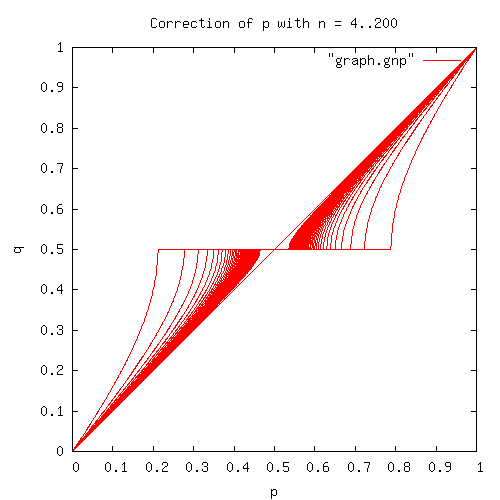
\includegraphics[scale=0.5]{graph.png}
\caption{
For a set of values for \(n\) (with \(n = 2\tilde{n}\)) ranging from \(4\) (farthest on the left and right) to \(200\) (nearest to \(f(p) = p\))}
\end{figure}

\newpage
\section{Code}
Finally we can put our results into a code:\\
\\
\ \ if(\ p\ \(<\){}\ 0.5$\ast$(1\ -{}\ sqrt(\ (2$\ast$\(\tilde{n}\)-{}2)\ /\ (2$\ast$\(\tilde{n}\)-{}1)\ ))\ )\\
\ \ \ \ q\ =\ 0.5\ $\ast$\ (1\ -{}\ sqrt(\ 4$\ast$p$\ast$(1-{}p)\ $\ast$\ (2$\ast$\(\tilde{n}\)-{}1)\ /\ (2$\ast$\(\tilde{n}\)-{}2)\ )\ );\\
\ \ else\\
\ \ if(\ p\ \(>\){}\ 0.5$\ast$(1\ +\ sqrt(\ (2$\ast$\(\tilde{n}\)-{}2)\ /\ (2$\ast$\(\tilde{n}\)-{}1)\ ))\ )\\
\ \ \ \ q\ =\ 0.5\ $\ast$\ (1\ +\ sqrt(\ 4$\ast$p$\ast$(1-{}p)\ $\ast$\ (2$\ast$\(\tilde{n}\)-{}1)\ /\ (2$\ast$\(\tilde{n}\)-{}2)\ )\ );\\
\ \ else\\
\ \ \ \ q\ =\ 0.5;\\
\ \\
or for the general formula with \(n \neq 2\tilde{n}\):\\
\\
\ \ if(\ p\ \(<\){}\ 0.5$\ast$(1\ -{}\ sqrt(\ (\(\tilde{n}\)-{}1)$\ast$n\ /\ ((n-{}1)$\ast$\(\tilde{n}\))\ )\ )\ )\\
\ \ \ \ q\ =\ 0.5\ $\ast$\ (1\ -{}\ sqrt(\ 4$\ast$p$\ast$(1-{}p)\ $\ast$\ (n-{}1)$\ast$\(\tilde{n}\)\ /\ ((\(\tilde{n}\)-{}1)$\ast$n)\ )\ );\\
\ \ else\\
\ \ if(\ p\ \(>\){}\ 0.5$\ast$(1\ +\ sqrt(\ (\(\tilde{n}\)-{}1)$\ast$n\ /\ ((n-{}1)$\ast$\(\tilde{n}\))\ )\ )\ )\\
\ \ \ \ q\ =\ 0.5\ $\ast$\ (1\ +\ sqrt(\ 4$\ast$p$\ast$(1-{}p)\ $\ast$\ (n-{}1)$\ast$\(\tilde{n}\)\ /\ ((\(\tilde{n}\)-{}1)$\ast$n)\ )\ );\\
\ \ else\\
\ \ \ \ q\ =\ 0.5;\\
\\

The main advantage of this code is that only minimal changes to the code have to be made because this way of reducing the diversity loss is problem independant (at least for bitstrings on a flat landscape in UDMA). The code has to be inserted just after determining the distribution \(p\).


\section{Multiple components}

If we set \(C > 1\), i.e. bitstrings longer than one bit, we will get similar results. While equation \(3\) does use \(C\) to determine the diversity of a generated population we can look at each component seperately as they are not connected in UMDA (in a flat fitness landscape). All bits belonging to one component in the population are created with an own distribution \(p\) that is independant from the other \(p\). Therefor we can handle a problem with \(C > 1\) like \(C\) seperate problems, each with one component.
How interconnected components would affect the diversity out of the scope of this paper and remains to be investigated.


\newpage
\section{Tests}

\subsection{General test configuration}

UMDA

\subsection{'Needle in a Haystack' problem}

flat fitness landscape

\subsection{OneMax problem}



\section{Conclusions}


\section{Fields of further research}

In the following chapter I will run several tests with different parameters. In the third chapter I will discuss further applications~

\begin{thebibliography}{99}
\bibitem{Shapiro} {\sc Shapiro, J.L.:}  \textit{Diversity loss in general estimation of distribution algorithms}, 2006.
\end{thebibliography}
\end{document}

